\section{Evaluation of PREF for traffic splitting}

An individual evaluation of PREF, the splitting mechanism of PREFLEX, is required to understand better the global performance of PREFLEX. Indeed, the two components PREF and LEX are functionally separate. Hence, in this section PREF will be disassociated from the rest of the architecture and put in two other contexts. A simplified load balancer, referred to in this text as “equalization mode”, that balances the traffic in a fixed and equal fraction over all the available paths. The second scenario, is in a simplified version of TEXCP that doesn't include the core routers based traffic shaping for congestion management. 

For both modes, we are going to use the topology ..,. The variation of the number pf flows in the system is kept simple with the same number of flows for both servers. Only one change was introduced to see how fast is the reaction of the algorithm. It concerns the number of flows for each destination.

\subsection{Equalization Mode}

In this mode each balancer defines an equal split over the three paths for each of the destination. Figure \ref{fig:fwnd} gives an example

 \begin{figure}[h]
  \begin{center}
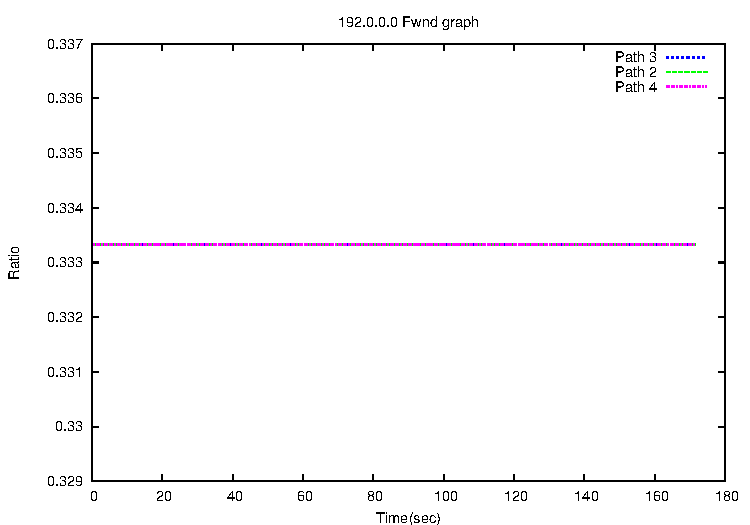
\epsfig{file=img/results/fwnd-192-0-0-0, width=4.5in}
\caption{
  Flowlet ratio $f_{i}$ for destination $E_{1}$ as set by ingress point $I_{1}$.
    \label{fig:fwnd}
}
 \end{center}
\end{figure}

The graphs bellow show the throughput of the traffic that ingress node I1 send over each link.\\

PREF

\begin{figure}[h]
 \begin{center}

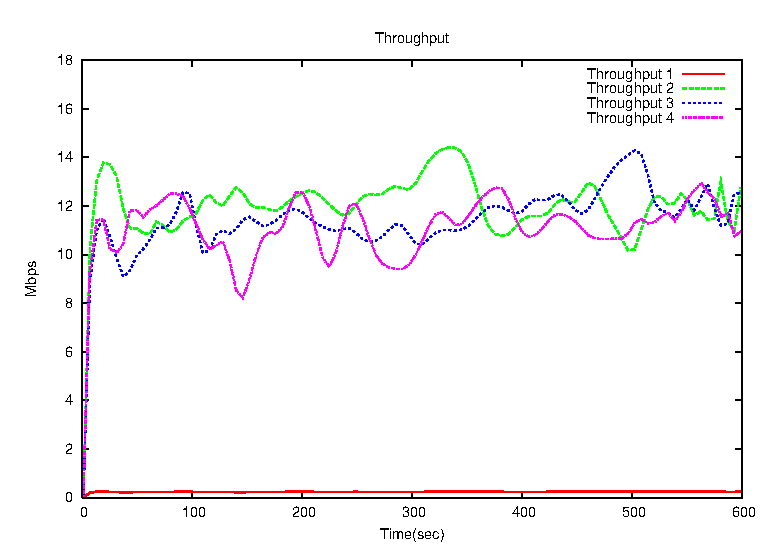
\epsfig{file=img/results/sec5-1/equalization-PREF/eleven/throuputs, width=4.5in}
\caption{
  Throughputs over each interface.
    \label{fig:equal-thro-pref}
}
\end{center}

FLARE

\end{figure}

 \begin{figure}[h!]
 \begin{center}
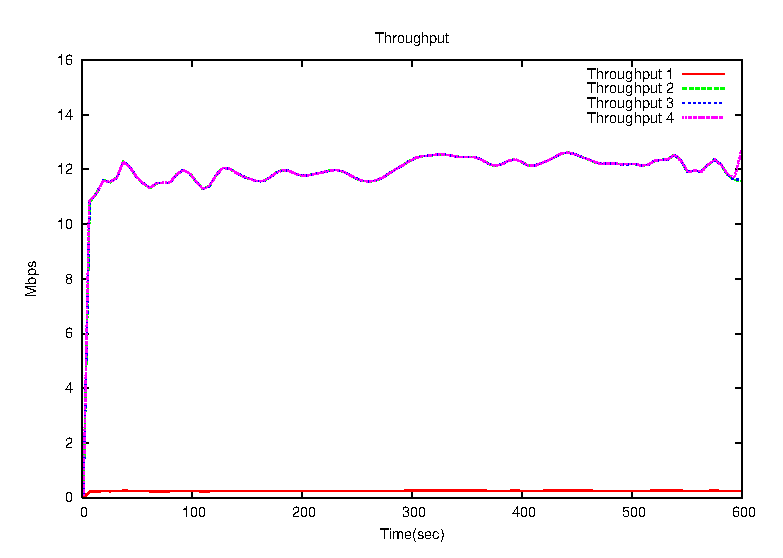
\epsfig{file=img/results/sec5-1/equalization-FLARE/eleven/throuputs, width=4.5in}
\caption{
  Throughputs over each interface.
    \label{fig:equal-thro-flare}
}
\end{center}

\end{figure}

%\begin{figure}[h]
%  \begin{center}
%    \mbox{
%      \subfigure[]{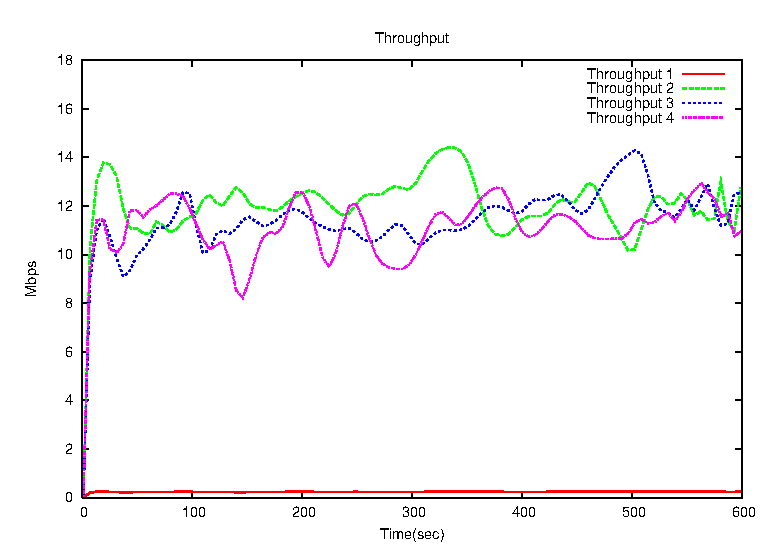
\includegraphics[width=4.0in]{img/results/sec5-1/equalization-PREF/eleven/throuputs}}\\
%      \subfigure[]{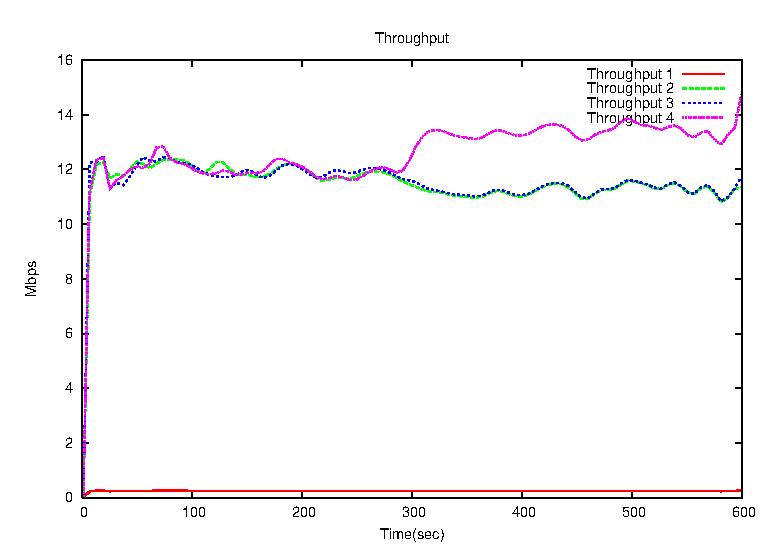
\includegraphics[width=4.0in]{file=img/results/sec5-1/equalization-FLARE/eleven/throuputs}}
%    }
%\caption{caption goes here.}
%\label{fig:parts}
%\end{center}
%\end{figure}

As expected, PREF which is equibalen a flow based traffic splitor, doesn't match the accuracy level of FLARE in splitting the traffic, but still the difference on the throughput over each path stays limited. The graphs also show oscillation behaviour of PREF. We find the same oscillation behaviour in the graphs of drop rate at the bottlenecks.

PREF

\begin{figure}[h]
 \begin{center}

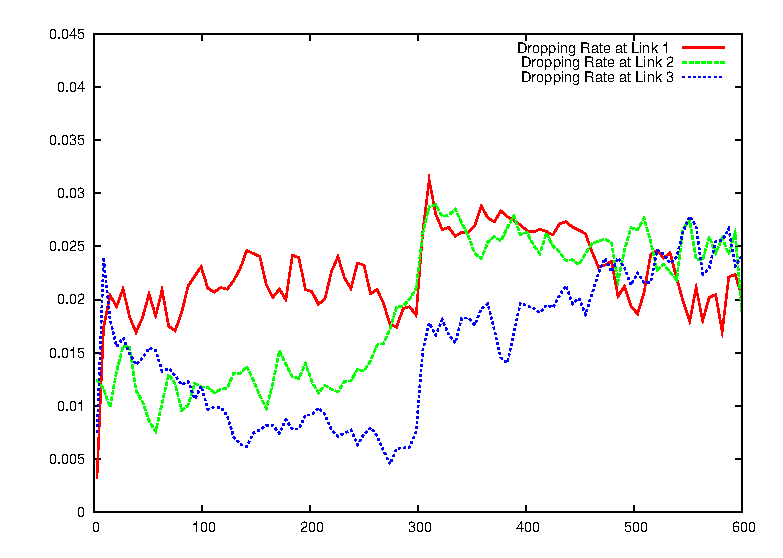
\epsfig{file=img/results/sec5-1/equalization-PREF/dropRate, width=4.5in}
\caption{
  Drop Rate at the botlenecks.
    \label{fig:equal-thro-pref}
}
\end{center}



\end{figure}
FLARE
 \begin{figure}[h!]
 \begin{center}
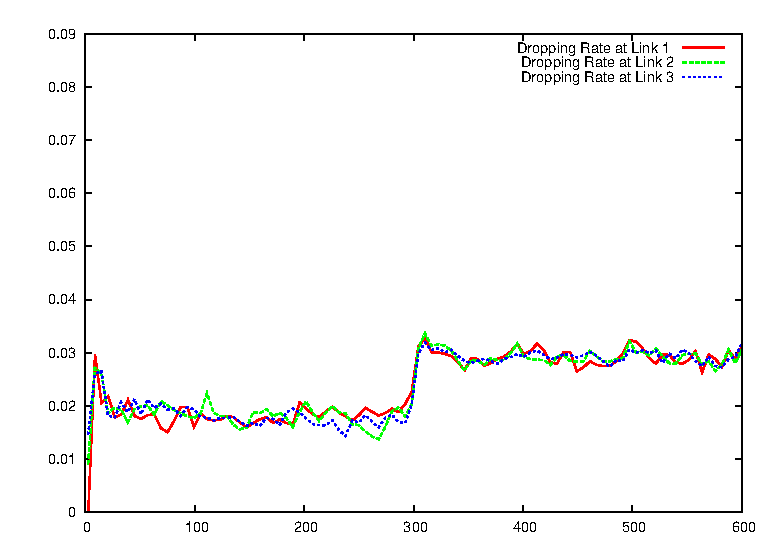
\epsfig{file=img/results/sec5-1/equalization-FLARE/dropRate, width=4.5in}
\caption{
  Drop Rate at the botlenecks.
    \label{fig:equal-thro-flare}
}
\end{center}

\end{figure}

These seconds graphs provide a hint about the reason of the fluctuation. The path assignement process of PREF makes the flowlets, which are transport aware, evolve their whole life cycle in one path and hence have a different congestion experience than the other flows. As a result, their tranmission rates and the congestion that they are making ares decorrelated.In the other hand, the network flowlets used by FLARE are a smaller order of granuilarity and makes that the transport flows get a path attributed multiple times during their flow time. As a result, the congestion level that a TCP routine experienced is a combination of the congestion in the different paths and hence the flows adapt their tranmission rate to a common level of congestion and the fluctuations are less significant.

%\clearpage

\subsection{balancing by path utilization}

Now we consider the example of balancing by path utilization, a simplified version of TEXCP where ingress points don't use the core routers feedback to control their transmissions rate.

PREF

\begin{figure}[h]
 \begin{center}

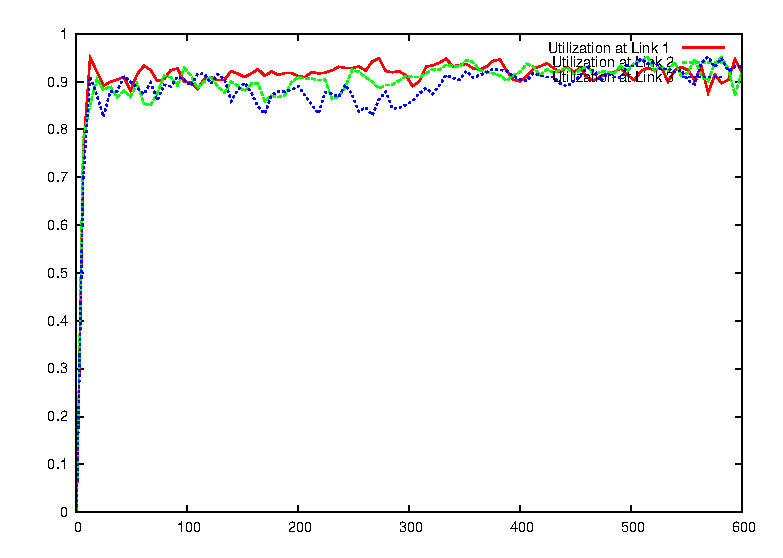
\epsfig{file=img/results/sec5-1/equalization-PREF/util, width=4.5in}
\caption{
  Path utilization measured at bottlenecks. 
    \label{fig:texcp-util-pref}
}
\end{center}

\end{figure}
FLARE
 \begin{figure}[h!]
 \begin{center}
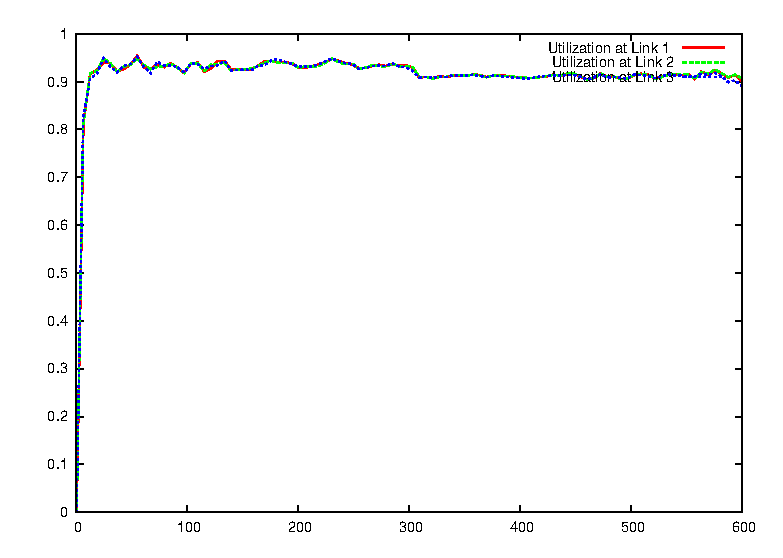
\epsfig{file=img/results/sec5-1/texcp-flare/util, width=4.5in}
\caption{
  Path utilization measured at bottlenecks. 
    \label{fig:texcp-util-flare}
}
\end{center}

\end{figure}

The previous analysis is stil valid ine the case of balamcing by path utilization. This last parameter oscillates in the case of PREF splitting, and equalization is not achieved with the same accuracy.

\paragraph{Conclusion}

Splitting traffic using PREF is required for the congestion mechanism defined by LEX. The revelation of a path congestion requires that the retranmitted packets follow the same path. Moreover, it makes congestion bakancing a bit more difficult since the flows follow one path with decorelated congestion experiences. However, PREF allows path diversity schemes at end hosts and network to coexist. The performance of PREF could be enhanced further, if efficient strategies of how and when to trigger path selection were deployed at by the recievers.
 
%\section{Load balancing VS congestion balancing}
\section{Analysis of PREFLEX balancing algorithm}

In this section we are going to evaluate the performance of the algorithm for different configuration parameters. 

\subsection{Decision time interval}

The decision time interval is an external parameter for the algorithm. It determines how often the network domain call to update the split. The raction of the algorithm and how long it takes to reach equilibrium is linked to the decision interval. But from another hand, this decision interval is also dependant of the period over which the loss signals are aggregated. As a result, a frequent update of the split may result in a unstability of the system that will be even stressed when the aggregation time of the losses is carried out for small periods of time. In practice, we choose the decision time interval to the double of the time value for the aggregation.

The graphs bellow show the dropping rate observed at the bottleneck. 

\begin{figure}[h]
 \begin{center}

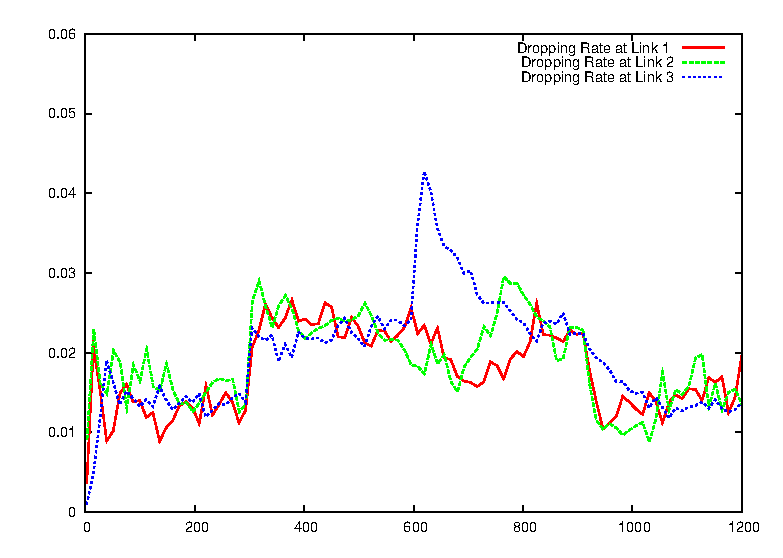
\epsfig{file=img/sec-5-2-1/eight/dropRate, width=4.5in}
\caption{
  Drop Rate at the botlenecks. (An 
    \label{fig:split-eight}
}
\end{center}
\end{figure}

%FLARE
 \begin{figure}[h!]
 \begin{center}
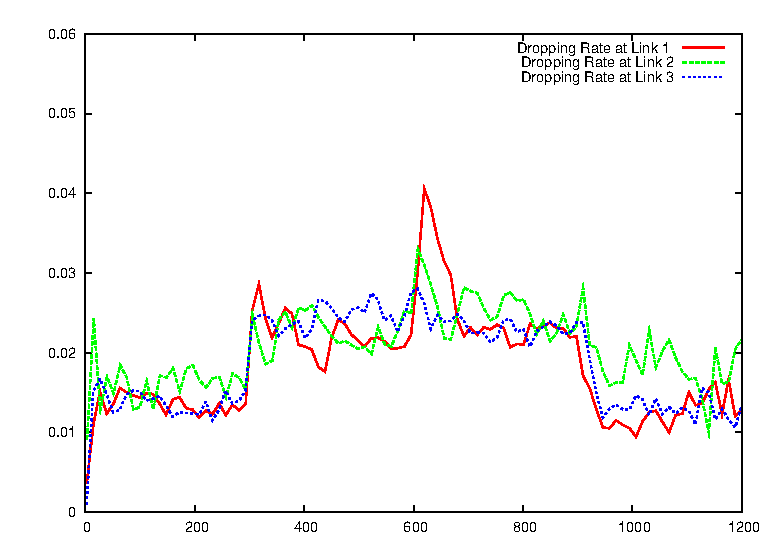
\epsfig{file=img/sec-5-2-1/four/dropRate, width=4.5in}
\caption{
  Drop Rate at the botlenecks.
    \label{fig:split-time-four}
}
\end{center}

\end{figure}

\clearpage

Eight

\begin{figure}[h]
 \begin{center}

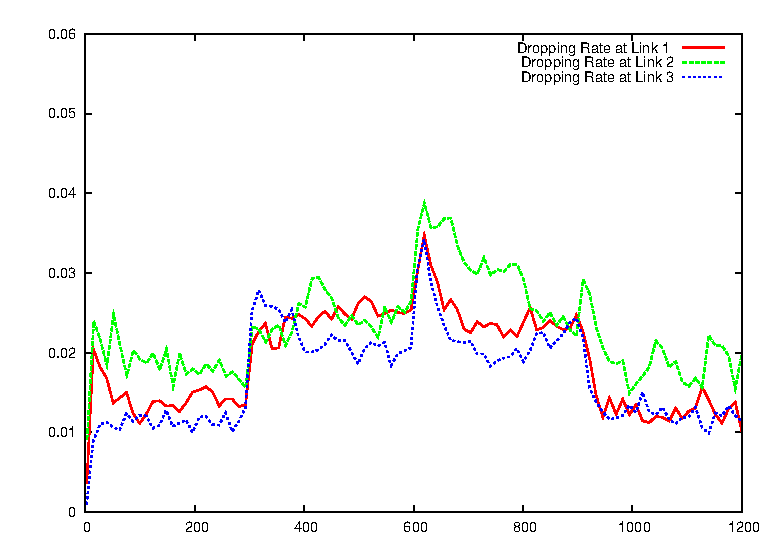
\epsfig{file=img/sec-5-2-1/one/dropRate, width=4.5in}
\caption{
  Drop Rate at the botlenecks.
    \label{fig:split-one}
}
\end{center}
\end{figure}

As expected, whith a small update interval the algorithm acts more aggresively and doesn't leave enough time for the flows to reach stability. As a result the congestion level experienced in the different paths (expressed by the dropping rate at each bottleneck) is not well balanced. A larger time intervals (8 and 4 sec) allow to achieve a better balancing of the congestion over the available paths and with an enhanced stability. From the different simulations that we've carried out, an update interval between 40 to 100 RTT (apprixmately 100ms for the simulations here) allowed to achieve most of the time a good accuracy of the congestion balancing. An even higher value for the update interval turns the balancer too slow. This effect could be illustrated with the reaction of the system for sudden and important change in traffic demand. We could see at around the second 600, when the demand on traffic turned from a destination to another one, the balancer with an update interval of 8 sec required relatively more time to achive equilibruim again.    
 
 

%\begin{figure}[htbp]
%\begin{center}
%\subfloat[]{
%\label{rcpstart4}
%\includegraphics[scale=0.4]{plots/lan/1.5Mb/rcp/flowstart4.eps}}
%\hspace{10mm}
%\subfloat[]{
%\label{xcprcpstart4}
%\includegraphics[scale=0.4]{plots/lan/1.5Mb/xcp0/flowstart4.eps}}
%\caption{The throughput of end-hosts and the router queue as a fourth flow starts, using \protect\subref{rcpstart4} RCP and \protect\subref{xcprcpstart4} XCP.}
%\label{rcpstart4comp}
%\end{center}
%\end{figure}

\subsection{Conservative policy}



\subsection{Equalization policy}

\section{Comparison between PREFLEX and TEXCP}